\documentclass[tikz,border=2mm]{standalone}

\begin{document}
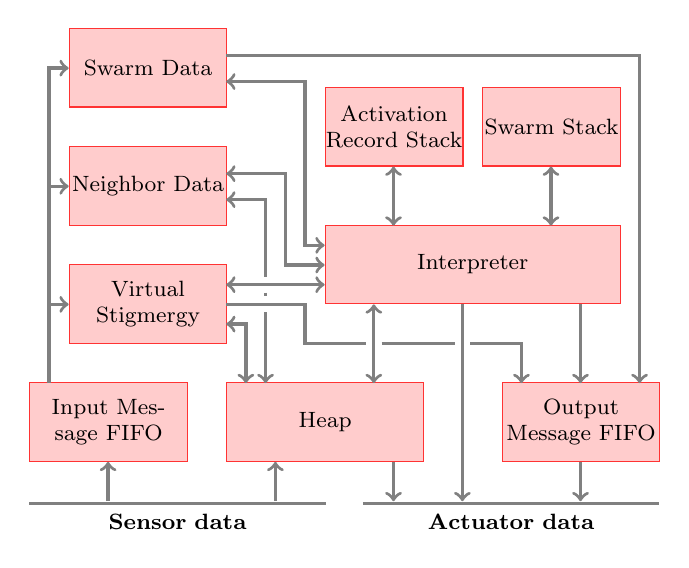
\begin{tikzpicture}[
  sensact/.style={inner sep=0,text width=3.75cm,minimum height=3ex,text centered,font=\footnotesize},
  module/.style={draw=red!80,fill=red!20,inner sep=0,minimum height=1cm,anchor=south west,text centered,font=\footnotesize},
  arr/.style={very thick,draw=black!50}
  ]
  % 
  % Sensor/actuator
  % 
  \node(sensor)  [sensact,anchor=south west] at (0,0) {\bf Sensor data};
  \node(actuator)[sensact,anchor=south east] at (8,0) {\bf Actuator data};
  \draw[arr] (sensor.north west) -- (sensor.north east);
  \draw[arr] (actuator.north west) -- (actuator.north east);
  % 
  % Nodes
  % 
  \node(inmsg) [text width=2   cm,module]at (0   cm,1   cm){Input Message FIFO};
  \node(heap)  [text width=2.5 cm,module]at (2.5 cm,1   cm){Heap};
  \node(outmsg)[text width=2   cm,module]at (6   cm,1   cm){Output Message FIFO};
  \node(vstig) [text width=2   cm,module]at (0.5 cm,2.5 cm){Virtual Stigmergy};
  \node(nbr)   [text width=2   cm,module]at (0.5 cm,4   cm){Neighbor Data};
  \node(swdata)[text width=2   cm,module]at (0.5 cm,5.5 cm){Swarm Data};
  \node(interp)[text width=3.75cm,module]at (3.75cm,3   cm){Interpreter};
  \node(astack)[text width=1.75cm,module]at (3.75cm,4.75cm){Activation Record Stack};
  \node(sstack)[text width=1.75cm,module]at (5.75cm,4.75cm){Swarm Stack};
  % 
  % Arrows
  % 
  % sensor -> inmsg
  \draw[arr,->] (1cm,0.5cm) -- (1cm,1cm);
  % sensor -> heap
  \draw[arr,->] (3.125cm,0.5cm) -- (3.125cm,1cm);
  % outmsg -> actuator
  \draw[arr,->] (7cm,1cm) -- (7cm,0.5cm);
  % heap -> actuator
  \draw[arr,->] (4.625cm,1cm) -- (4.625cm,0.5cm);
  % inmsg -> swdata
  \draw[arr,->] (0.25cm,2cm) |- (0.5cm,6cm);
  % inmsg -> vstig
  \draw[arr,->] (0.25cm,3cm) -- (0.5cm,3cm);
  % inmsg -> nbr
  \draw[arr,->] (0.25cm,4.5cm) -- (0.5cm,4.5cm);
  % vstig <-> interp
  \draw[arr,<->] (2.5cm,3.25cm) -- (3.75cm,3.25cm);
  % vstig <-> heap
  \draw[arr,<->] (2.5cm,2.75cm) -|(2.75cm,2cm);
  % nbr <-> interp
  \draw[arr,<->] (2.5cm,4.66cm) -- (3.25cm,4.66cm) -- (3.25cm,3.5cm) -- (3.75cm,3.5cm);
  % nbr <-> heap
  \draw[arr,<-] (2.5cm,4.33cm) -| (3cm,3.35cm);
  \draw[arr,]   (3cm,3.15cm) -- (3cm,3.1cm);
  \draw[arr,->] (3cm,2.9cm) -- (3cm,2cm);
  % swdata <-> interp
  \draw[arr,<->] (2.5cm,5.83cm) -- (3.5cm,5.83cm) -- (3.5cm,3.75cm) -- (3.75cm,3.75cm);
  % astack <-> interp
  \draw[arr,<->] (4.625cm,4.75cm) -- (4.625cm,4cm);
  % sstack <-> interp
  \draw[arr,<->] (6.625cm,4.75cm) -- (6.625cm,4cm);
  % swdata -> outmsg
  \draw[arr,->] (2.5cm,6.16cm) -| (7.75cm,2cm);
  % interp -> actuators
  \draw[arr,->] (5.5cm,3cm) -- (5.5cm,0.5cm);
  % interp -> outmsg
  \draw[arr,->] (7cm,3cm) -- (7cm,2cm);
  % interp <-> heap
  \draw[arr,<->] (4.375cm,3cm) -- (4.375cm,2cm);
  % vstig -> outmsg
  \draw[arr] (2.5cm,3cm) -- (3.5cm,3cm) -- (3.5cm,2.5cm) -- (4.275cm,2.5cm);
  \draw[arr] (4.475cm,2.5cm) -- (5.4cm,2.5cm);
  \draw[arr,->] (5.6cm,2.5cm) -- (6.25cm,2.5cm) -- (6.25cm,2cm);
\end{tikzpicture}
\end{document}
